\documentclass[a4paper]{article}
\usepackage{geometry}
\usepackage{graphicx}
\usepackage{natbib}
\usepackage{amsmath}
\usepackage{amssymb}
\usepackage{amsthm}
\usepackage{paralist}
\usepackage{epstopdf}
\usepackage{tabularx}
\usepackage{longtable}
\usepackage{multirow}
\usepackage{multicol}
\usepackage[hidelinks]{hyperref}
\usepackage{fancyvrb}
\usepackage{algorithm}
\usepackage{algorithmic}
\usepackage{float}
\usepackage{paralist}
\usepackage[svgname]{xcolor}
\usepackage{enumerate}
\usepackage{array}
\usepackage{times}
\usepackage{url}
\usepackage{fancyhdr}
\usepackage{comment}
\usepackage{environ}
\usepackage{times}
\usepackage{textcomp}
\usepackage{caption}


\urlstyle{rm}

\setlength\parindent{0pt} % Removes all indentation from paragraphs
\theoremstyle{definition}
\newtheorem{definition}{Definition}[]
\newtheorem{conjecture}{Conjecture}[]
\newtheorem{example}{Example}[]
\newtheorem{theorem}{Theorem}[]
\newtheorem{lemma}{Lemma}
\newtheorem{proposition}{Proposition}
\newtheorem{corollary}{Corollary}

\floatname{algorithm}{Procedure}
\renewcommand{\algorithmicrequire}{\textbf{Input:}}
\renewcommand{\algorithmicensure}{\textbf{Output:}}
\newcommand{\abs}[1]{\lvert#1\rvert}
\newcommand{\norm}[1]{\lVert#1\rVert}
\newcommand{\RR}{\mathbb{R}}
\newcommand{\CC}{\mathbb{C}}
\newcommand{\Nat}{\mathbb{N}}
\newcommand{\br}[1]{\{#1\}}
\DeclareMathOperator*{\argmin}{arg\,min}
\DeclareMathOperator*{\argmax}{arg\,max}
\renewcommand{\qedsymbol}{$\blacksquare$}

\definecolor{dkgreen}{rgb}{0,0.6,0}
\definecolor{gray}{rgb}{0.5,0.5,0.5}
\definecolor{mauve}{rgb}{0.58,0,0.82}

\newcommand{\Var}{\mathrm{Var}}
\newcommand{\Cov}{\mathrm{Cov}}

\newcommand{\vc}[1]{\boldsymbol{#1}}
\newcommand{\xv}{\vc{x}}
\newcommand{\Sigmav}{\vc{\Sigma}}
\newcommand{\alphav}{\vc{\alpha}}
\newcommand{\muv}{\vc{\mu}}

\newcommand{\red}[1]{\textcolor{red}{#1}}

\def\x{\mathbf x}
\def\y{\mathbf y}
\def\w{\mathbf w}
\def\v{\mathbf v}
\def\E{\mathbb E}
\def\V{\mathbb V}

% TO SHOW SOLUTIONS, include following (else comment out):
\newenvironment{soln}{
    \leavevmode\color{blue}\ignorespaces
}{}


\hypersetup{
%    colorlinks,
    linkcolor={red!50!black},
    citecolor={blue!50!black},
    urlcolor={blue!80!black}
}

\geometry{
  top=1in,            % <-- you want to adjust this
  inner=1in,
  outer=1in,
  bottom=1in,
  headheight=3em,       % <-- and this
  headsep=2em,          % <-- and this
  footskip=3em,
}


\pagestyle{fancyplain}
\lhead{\fancyplain{}{Homework 1: Background Test}}
\rhead{\fancyplain{}{CS 760 Machine Learning}}
\cfoot{\thepage}

\title{\textsc{Homework 1: \\ Background Test}} % Title

%\newcommand{\outDate}{Aug. 31, 2016}
%\newcommand{\dueDate}{5:30 pm, Sep. 7, 2016}


%%% NOTE:  Replace 'NAME HERE' etc., and delete any "\red{}" wrappers (so it won't show up as red)

\author{
Wenyan Zhou \\
9077005776\\
} 

\date{}

\begin{document}

\maketitle 


% \textbf{Instructions:} \text{Submit your homework} on time 
  % by submitting \textbf{BOTH} a hard-copy to the hanging folders outside Sandra Winkler's 
  % office (GHC 8221) \textbf{AND} electronically
  % to \href{https://www.gradescope.com}{Gradescope}.  For Gradescope, you 
  % will need to specify which pages go with which question.  Please submit
  % Sections 1 through 4 to Q1, Sections 5 through 6.3 to Q2, and Sections
  % 6.4 to 8 to Q3.  We provide a LaTeX template in which you can use to
  % type up your solutions.  This template ensures the correct sections
  % start on new pages.  Please check Piazza for updates about the homework.
\begin{center}
\Huge
Minimum Background Test [80 pts]
\end{center}

\section{Vectors and Matrices [20 pts]}
Consider the matrix $X$ and the vectors $\mathbf{y}$ and $\textbf{z}$ below:
$$
X = \begin{pmatrix}
9 & 8 \\ 7 & 6 \\
\end{pmatrix}
\qquad \mathbf{y} = \begin{pmatrix}
9 \\ 8
\end{pmatrix} \qquad \mathbf{z} = \begin{pmatrix}
7 \\ 6
\end{pmatrix}
$$
\begin{enumerate}
	\item 	What is the inner product of the vectors $\mathbf{y}$ and $\mathbf{z}$? (this is also sometimes called the \emph{dot product}, and is sometimes written as $\mathbf{y}^T\mathbf{z}$)\\
	    \begin{soln} 
	    $$
	    \mathbf{y}^T\mathbf{z} = \begin{pmatrix}
	    9 & 8 \\
	    \end{pmatrix}
	    \begin{pmatrix}
	    7 \\
	    6 \\
	    \end{pmatrix}
	    = 111
	    $$
	    \end{soln}
	\item 	What is the product $X\mathbf{y}$?\\
	    \begin{soln}
	    $$
	    X\mathbf{y} = \begin{pmatrix}
	    9 & 8 \\ 
	    7 & 6 \\
	    \end{pmatrix}
	     \begin{pmatrix}
	    9 \\
	    8 \\
	    \end{pmatrix}
	    = \begin{pmatrix}
	    145 \\
	    111 \\
	    \end{pmatrix}
	    $$  
	    \end{soln}
	\item 	Is $X$ invertible? If so, give the inverse, and if no, explain why not.\\
        \begin{soln}  
        Yes. \\
        Let $$
        X^{-1}X = I,
        $$
        then $$
        X^{-1} = \begin{pmatrix}
        -3 & 4 \\
        3.5 & -4.5
        \end{pmatrix}
        $$
        \end{soln}
	\item 	What is the rank of $X$?\\
	    \begin{soln}  
	    $$
	    |X| = \begin{vmatrix}
	    9 & 8 \\
	    7 & 6 \\
	    \end{vmatrix}
	    = -2 \neq 0
	    $$
	    Therefore, the rank of X is 2.
	    \end{soln}
\end{enumerate}


\section{Calculus [20 pts]}
\begin{enumerate}
	\item 	If $y = 4x^3 - x^2 + 7$ then what is the derivative of $y$ with respect to $x$?\\
	\begin{soln}
	$$
	\frac{dy}{dx} = 12x^{2} - 2x
	$$
	\end{soln}
	\item If $y = \tan(z)x^{6z} - \ln(\frac{7x + z}{x^{4}})$, what is the partial derivative of $y$ with respect to $x$?\\
	\begin{soln}
	\begin{equation*}
	\begin{aligned}
	\frac{\partial y}{\partial x} &= 6ztan(z)x^{6z-1} - \frac{x^{4}}{7x+z}\frac{7x^4-4x^3(7x+z)}{x^8} \\
	                                        &= 6ztan(z)x^{6z-1} - \frac{-21x^4-4zx^3}{7x^5+zx^4} \\
	                                        &= 6ztan(z)x^{6z-1} + \frac{21x+4z}{7x^2+zx}
	\end{aligned}
	\end{equation*}
	\end{soln}
\end{enumerate}




\section{Probability and Statistics [20 pts]}
Consider a sample of data $S = \{0, 1, 1, 0, 0, 1, 1\}$ created by flipping a coin $x$ seven times, where 0 denotes that the coin turned up heads and 1 denotes that it turned up tails.
\begin{enumerate}
	\item 	What is the sample mean for this data?\\
	    \begin{soln}
	    $$
	    \bar{x} = (0+1+1+0+0+1+1)/7 = \frac{4}{7}
	    $$
	    \end{soln}
	\item 	What is the sample variance for this data?\\
	    \begin{soln}
	    $$
	    S^2 = [3\times(0-\frac{4}{7})^2 + 4\times(1-\frac{4}{7})^2]/6 = \frac{2}{7}
	    $$
	    \end{soln}
	\item 	What is the probability of observing this data, assuming it was generated by flipping a biased coin with $p(x=1) = 0.7, p(x=0) = 0.3$.\\
	    \begin{soln}
	    $$
	    p(3H, 4T) = \begin{pmatrix}
	    7 \\
	    3 \\
	    \end{pmatrix}
	    \times 0.3^3 \times 0.7^4 = 0.2268945
	    $$
	    \end{soln}
	\item 	Note that the probability of this data sample would be greater if the value of $p(x = 1)$ was not $0.7$, but instead some other value. What is the value that maximizes the probability of the sample $S$? Please justify your answer.\\
	    \begin{soln}
	    Suppose $p(x=1) = p$,\\
	    the probability of observing S is $p(3H, 4T) = \begin{pmatrix}
	    7 \\
	    3 \\
	    \end{pmatrix}
	    \times p^4(1-p)^3
	    $. \\
	    To maximize the value($p \neq 0$), $p = \frac{4}{7}$.\\
	    Then, $p(3H,4T) = 0.2937552$
	    \end{soln}
	\item 	Consider the following joint probability table where both $A$ and $B$ are binary random variables: 
\begin{table}[htb]
\centering
	\begin{tabular}{ccc}\hline
	A & B & $P(A, B)$  \\\hline
	0 & 0 & 0.1 \\
	0 & 1 & 0.4 \\
	1 & 0 & 0.2 \\
	1 & 1 & 0.3 \\\hline
	\end{tabular}
\end{table}
\begin{enumerate}
	\item 	What is $P(A = 0, B = 0)$?\\
	    \begin{soln} 
	    $$P(A = 0, B = 0) = 0.1$$
	    \end{soln}
	\item 	What is $P(A = 1)$?\\
	    \begin{soln}
	    $$P(A = 1) = P(A = 1, B = 0) + P(A = 1, B = 1) = 0.2 + 0.3 = 0.5$$
	    \end{soln}
	\item 	What is $P(A = 0 | B = 1)$?\\
	    \begin{soln}
	    $$P(A = 0 | B = 1) = \frac{P(A = 0, B = 1)}{P(B = 1)} = 0.4/(0.4 + 0.3) = \frac{4}{7}$$
	    \end{soln}
	\item 	What is $P(A = 0 \vee B = 0 )$?\\
	    \begin{soln}
	    $$P(A = 0 \vee B = 0) = 1 - P(A = 1, B = 1) = 1 - 0.3 = 0.7$$
	    \end{soln}
\end{enumerate}
\end{enumerate}


\section{Big-O Notation [20 pts]}
For each pair $(f, g)$ of functions below, list which of the following
are true: $f(n) = O(g(n))$, $g(n) = O(f(n))$, both, or
neither. Briefly justify your answers.
\begin{enumerate}
	\item 	$f(n) = \frac{n}{2}$, $g(n) = \log_{2}(n)$.\\
	    \begin{soln}
	    $g(n) = O(f(n))$ \\
	    Because
	    $$
	    { \lim_{n \to \infty} sup|\frac{g(n)}{f(n)}|} = { \lim_{n \to \infty} sup|\frac{log_2(n)}{n/2}|} 
	    = { \lim_{n \to \infty} sup|\frac{(1/n)(1/ln2)}{1/2}|} = { \lim_{n \to \infty} sup|\frac{2}{nln2}|} < \infty
	    $$ \\
	    $$
	    { \lim_{n \to \infty} sup|\frac{f(n)}{g(n)}|} = { \lim_{n \to \infty} sup|\frac{nln2}{2}|} = \infty
	    $$
	    \end{soln}
	\item 	$f(n) = \ln(n)$, $g(n) = \log_{2}(n)$.\\
	    \begin{soln}
	    Both $f(n) = O(g(n))$ and $g(n) = O(f(n))$\\
	    Because
	    $$
	    { \lim_{n \to \infty} sup|\frac{f(n)}{g(n)}|} = { \lim_{n \to \infty} sup|\frac{lnn}{log_2(n)}|} 
	    = { \lim_{n \to \infty} sup|\frac{1/n}{(1/n)(1/ln2)}|} = ln2 < \infty
	    $$
	    $$
	    { \lim_{n \to \infty} sup|\frac{g(n)}{f(n)}|} = \frac{1}{ln2} < \infty
	    $$
	    \end{soln}
	\item 	$f(n) = n^{100}$, $g(n) = 100^n$.\\
	    \begin{soln}
	    $f(n) = O(g(n))$ \\
	    Because
	    $$
	    { \lim_{n \to \infty} sup|\frac{f(n)}{g(n)}|} = { \lim_{n \to \infty} sup|\frac{n^{100}}{100^n}|} 
	    = { \lim_{n \to \infty} sup|\frac{100!}{(ln100)^{100}100^n}|} < \infty
	    $$ \\
	    $$
	    { \lim_{n \to \infty} sup|\frac{g(n)}{f(n)}|} = { \lim_{n \to \infty} sup|\frac{100^n}{n^{100}}|} 
	    = { \lim_{n \to \infty} sup|\frac{(ln100)^{100}100^n}{100!}|}= \infty
	    $$
	    \end{soln}
\end{enumerate}


\clearpage  % do not erase this!



\begin{center}
\Huge
Medium Background Test [20 pts]
\end{center}

\section{Algorithm [5 pts]}
\textbf{Divide and Conquer}: Assume that you are given a sorted array
with $n$ integers in the range $[-10, +10]$. Note that some integer values
may appear multiple times in the array. Additionally, you are
told that somewhere in the array the integer $0$ appears exactly once. Provide an
algorithm to locate the $0$ which runs in $O(\log(n))$. Explain your
algorithm in words, describe why the algorithm is correct, and justify
its running time.\\

\begin{soln}
Begin with dividing the whole array in half. If the middle of the interval is 0, we find it; else if 0 is less than the number in the middle of the interval, narrow the interval to the lower half; otherwise, narrow it to the upper half. Repeat the above steps until 0 is found. To justify the running time t, $2^t = n$, and $t = log_2(n) = log(n)/log(2) = O(log(n))$
\end{soln}

\section{Probability and Random Variables [5 pts]}
\subsection{Probability}
State true or false. Here $\Omega$ denotes the sample space and $A^c$ denotes the complement of the event $A$.
\begin{enumerate}
\item For any $A, B \subseteq \Omega$, $P(A|B)P(B) = P(B|A)P(A)$.\\
  \begin{soln}
  True.\\
  $$P(A|B)P(B) = P(A,B) = P(B|A)P(A)$$
  \end{soln}
\item For any $A, B \subseteq \Omega$, $P(A \cup B) = P(A) + P(B) - P(A | B)$.\\         
  \begin{soln}
  False.\\
  $$P(A \cup B) = P(A) + P(B) - P(A \cap B)$$
  \end{soln}
\item For any $A, B, C \subseteq \Omega$ such that $P(B \cup C) > 0$,
  $\frac{P(A \cup B \cup C)}{P(B \cup C)} \geq P(A | B \cup C) P(B \cup C)$.\\ 
  \begin{soln}
  True.\\
  $$\frac{P(A \cup B \cup C)}{P(B \cup C)} \geq P(A \cup B \cup C) \geq P(A \cap (B \cup C)) = P(A | B \cup C) P(B \cup C)$$.
  \end{soln}
\item For any $A, B\subseteq\Omega$ such that $P(B) > 0, P(A^c) > 0$,
  $P(B|A^C) + P(B|A) = 1$.\\ 
  \begin{soln}
  False.\\
  Suppose $B \subseteq A$, and $P(B) < P(A)$, then $P(B|A^C) + P(B|A) = P(B|A) = P(AB)/P(A) < 1$
  \end{soln}
\item For any $n$ events $\{A_i\}_{i=1}^n$, if
  $P(\bigcap_{i=1}^n A_i) = \sum_{i=1}^n P(A_i)$, then
  $\{A_i\}_{i=1}^n$ are mutually independent.\\
  \begin{soln}
  True.\\
  $P(\bigcap_{i=1}^n A_i) = \sum_{i=1}^n P(A_i)$, which indicates $P(A_i) = 0$ for all $A_i$. then $\{A_i\}_{i=1}^n$ are mutually independent.
  \end{soln}
\end{enumerate}

\subsection{Discrete and Continuous Distributions}
Match the distribution name to its probability density / mass
function. Below, $|\xv| = k$.
\begin{enumerate}[(a)]
\begin{minipage}{0.3\linewidth}
    \item Laplace \begin{soln} (h) \end{soln}
    \item Multinomial \begin{soln} (i) \end{soln}
    \item Poisson \begin{soln} (l) \end{soln}
    \item Dirichlet \begin{soln} (k) \end{soln}
    \item Gamma \begin{soln} (j) \end{soln}
\end{minipage}
\begin{minipage}{0.5\linewidth}
    \item $f(\xv; \Sigmav, \muv) = \frac{1}{\sqrt{(2\pi)^k \Sigmav}} \exp\left( -\frac{1}{2}
        (\xv - \muv)^T \Sigmav^{-1} (\xv - \muv)  \right)$
    \item $f(x; n, \alpha) = \binom{n}{x} \alpha^x (1 - \alpha)^{n-x}$
      for $x \in \{0,\ldots, n\}$; $0$ otherwise
    \item $f(x; b, \mu) = \frac{1}{2b} \exp\left( - \frac{|x - \mu|}{b} \right)$
    \item $f(\xv; n, \alphav) = \frac{n!}{\Pi_{i=1}^k x_i!}
      \Pi_{i=1}^k \alpha_i^{x_i}$ for $x_i \in \{0,\ldots,n\}$ and
      $\sum_{i=1}^k x_i = n$; $0$ otherwise
    \item $f(x; \alpha, \beta) = \frac{\beta^{\alpha}}{\Gamma(\alpha)} x^{\alpha -
        1}e^{-\beta x}$ for $x \in (0,+\infty)$; $0$ otherwise
    \item $f(\xv; \alphav) = \frac{\Gamma(\sum_{i=1}^k
        \alpha_i)}{\prod_{i=1}^k \Gamma(\alpha_i)} \prod_{i=1}^{k}
      x_i^{\alpha_i - 1}$ for $x_i \in (0,1)$ and $\sum_{i=1}^k x_i =
      1$; 0 otherwise
    \item $f(x; \lambda) = \lambda^x \frac{e^{-\lambda}}{x!}$ for all
      $x \in Z^+$; $0$ otherwise
\end{minipage}
\end{enumerate}
        
\subsection{Mean and Variance}
\begin{enumerate}
\item Consider a random variable which follows a Binomial
  distribution: $X \sim \text{Binomial}(n, p)$.
  \begin{enumerate}
  \item What is the mean of the random variable?\\
    \begin{soln}
    $$\mathbb{E}[X] = np$$
    \end{soln}
  \item What is the variance of the random variable?\\
    \begin{soln}
    $$\Var(X) = np(1-p)$$
    \end{soln}
  \end{enumerate}

\item Let $X$ be a random variable and
  $\mathbb{E}[X] = 1, \Var(X) = 1$. Compute the following values:
  \begin{enumerate}
  \item $\mathbb{E}[3X]$\\
    \begin{soln}
    $$\mathbb{E}[3X] = 3\mathbb{E}[X] = 3$$
    \end{soln}
  \item $\Var(3X)$\\
    \begin{soln}
    $$\Var(3X) = 9\Var(X) = 9$$
    \end{soln}
  \item $\Var(X+3)$\\
    \begin{soln}
    $$\Var(X+3) = \Var(X) = 1$$
    \end{soln}
  \end{enumerate}
\end{enumerate}

%\clearpage

\subsection{Mutual and Conditional Independence}
\begin{enumerate}
\item If $X$ and $Y$ are independent random variables, show that
  $\mathbb{E}[XY] = \mathbb{E}[X]\mathbb{E}[Y]$.
  
  \begin{soln}
  Take continuous variables as an example, it is the same for discrete variables.
  \begin{equation*}
  \begin{aligned}
  \mathbb{E}[XY] &= \int_{-\infty}^{+\infty}\int_{-\infty}^{+\infty}xyf(x,y)dxdy = \int_{-\infty}^{+\infty}\int_{-\infty}^{+\infty}xyf(x)f(y)dxdy \\
  &= \int_{-\infty}^{+\infty}xf(x)dx\int_{-\infty}^{+\infty}yf(y)dy = \mathbb{E}[X]\mathbb{E}[Y]
  \end{aligned}
  \end{equation*}
  \end{soln}
  
\item If $X$ and $Y$ are independent random variables, show that
  $\Var(X+Y) = \Var(X) + \Var(Y)$. \\
  Hint: $\Var(X+Y) = \Var(X) + 2\Cov(X, Y) + \Var(Y)$
  
  \begin{soln}
  \begin{equation*}
  \begin{aligned}
  \Var(X+Y) &= \Var(X) + 2Cov(X,Y) + \Var(Y) \\ 
  &= \Var(X) + 2[\mathbb{E}(XY) - \mathbb{E}(X)\mathbb{E}(Y)] + \Var(Y) \\ 
  &= \Var(X) + \Var(Y)
  \end{aligned}
  \end{equation*}
  \end{soln}
 
\item If we roll two dice that behave independently of each
  other, will the result of the first die tell us something about the
  result of the second die? 
  
  \begin{soln}
  No. Because the two events are independent.
  \end{soln}
  
  If, however, the first die's result is a 1,
  and someone tells you about a third event --- that the sum of the two
  results is even --- then given this information is the result of the second die
  independent of the first die? 
  
  \begin{soln}
  No. The third event indicates that the second die's result is 1 given the first die's result is 1, so that the sum of the two results is even.
  \end{soln}
\end{enumerate}

\subsection{Law of Large Numbers and the Central Limit Theorem}
Provide one line justifications.
\begin{enumerate}
\item Suppose we simultaneously flip two independent fair coins (i.e., the probability of heads is $1/2$ for each coin)
  and record the result. After 40,000 repetitions, the number
  of times the result was two heads is close to 10,000.  (Hint: calculate how close.)
  
  \begin{soln}
  According to LLN, $\bar{X}_n \overset{P}{\longrightarrow} \mu$ when $n \longrightarrow \infty$, because$\mu = \frac{1}{4}$, the number of two heads results is close to 10,000 for 40,000 repetitions.
  \end{soln}
  
\item Let $X_i\sim\mathcal{N}(0, 1)$ and $\bar{X} = \frac{1}{n}\sum_{i=1}^n X_i$, then the distribution of $\bar{X}$ satisfies 
  $$\sqrt{n}\bar{X}\overset{n\rightarrow\infty}{\longrightarrow}\mathcal{N}(0, 1)$$
  \begin{soln}
  According to CLT, $\sqrt{n}(\bar{X}-\mu)\overset{n\rightarrow\infty}{\longrightarrow}\mathcal{N}(0, \sigma^2)$, $\mathbb{E}(X_i) = \mu = 0$, $\Var(X_i) = \sigma^2 = 1$, thus proved.
  \end{soln}
  
\end{enumerate}



\section{Linear algebra [5 pts]}


\subsection{Norm-enclature}
Draw the regions corresponding to vectors $\mathbf{x}\in\RR^2$ with the following norms:
\begin{enumerate}
	\item 	$||\mathbf{x}||_1\leq 1$ (Recall that $||\mathbf{x}||_1 = \sum_i |x_i|$)
	\item 	$||\mathbf{x}||_2 \leq 1$ (Recall that $||\mathbf{x}||_2 =\sqrt{\sum_i x_i^2}$)
	\item 	$||\mathbf{x}||_\infty \leq 1$ (Recall that $||\mathbf{x}||_\infty = \max_i |x_i|$)
	
	\begin{soln}
	    %    (this can be done by highlighting text and pressing "cmd + /" for sharelatex+mac)
	   \begin{figure}[h!]	   
	       \centering
	       \begin{minipage}[c]{0.3\textwidth}
	       \centering
	       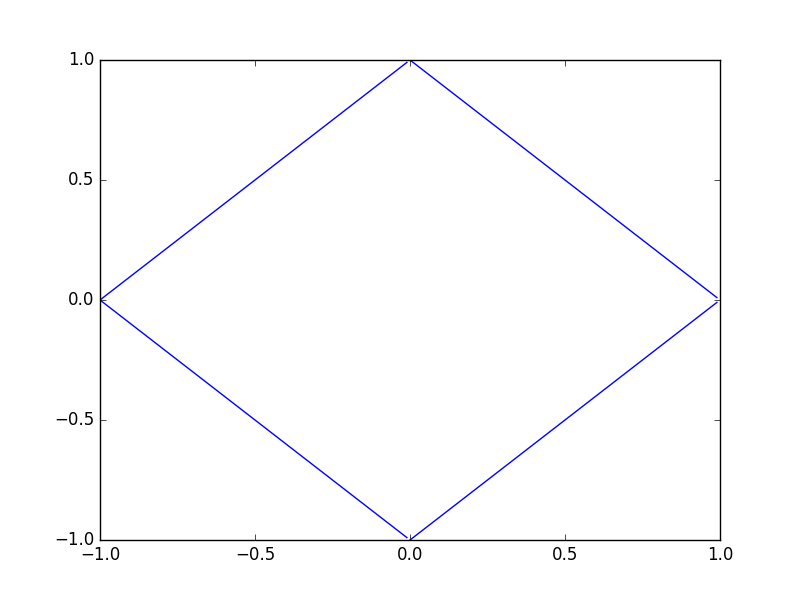
\includegraphics[width=0.8\textwidth,height=0.8\textwidth]{hw1_7_1_1.png}  
	       \captionsetup{labelformat=empty}
	       \caption{fig 7.1.1}
	       \label{fig:7.1.1}
	       \end{minipage}
	       \hfill
	       \begin{minipage}[c]{0.3\textwidth}
	       \centering
	       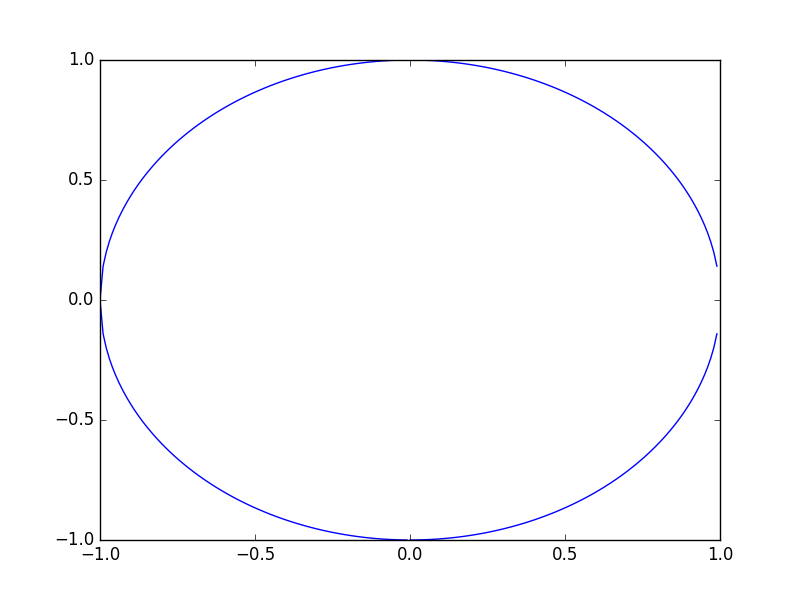
\includegraphics[width=0.8\textwidth,height=0.8\textwidth]{hw1_7_1_2.png}  
	       \captionsetup{labelformat=empty}
	       \caption{fig 7.1.2}
	       \label{fig:7.1.2}
	       \end{minipage}
	       \hfill
               \begin{minipage}[c]{0.3\textwidth}
               \centering
	       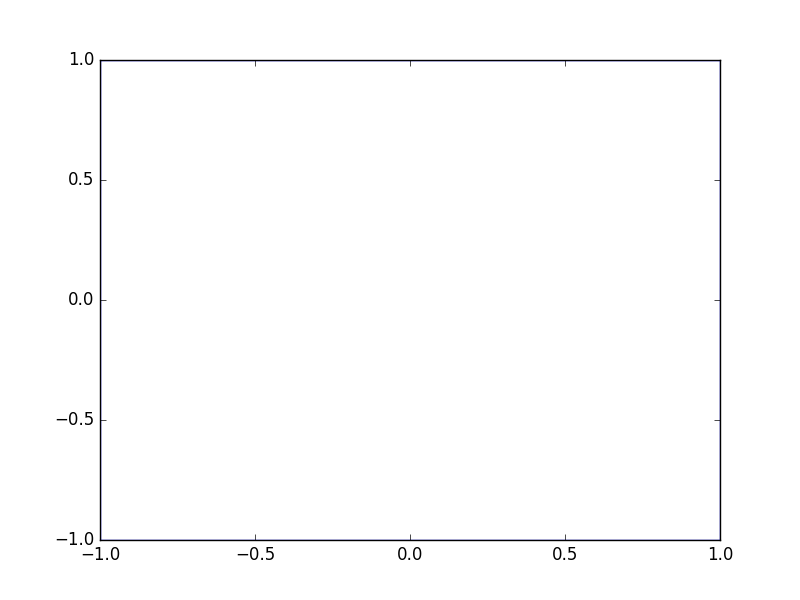
\includegraphics[width=0.8\textwidth,height=0.8\textwidth]{hw1_7_1_3.png}  
	       \captionsetup{labelformat=empty}
	       \caption{fig 7.1.3}
	       \label{fig:7.1.3}
	       \end{minipage}
	   \end{figure}


	\end{soln}
\end{enumerate}




\subsection{Geometry}
Prove that these are true or false. Provide all steps.
\begin{enumerate}
\item 	The smallest Euclidean distance from the origin to some point $\mathbf{x}$ in the hyperplane $\mathbf{w}^T\mathbf{x} + b = 0$ is $\frac{|b|}{||\mathbf{w}||_2}$.\\
\begin{soln}
True.\\ 
Suppose the projection of origin $\mathbf{x_0} = (0,0,...,0)_n$ on the hyperplane is $\mathbf{x_1} = (x_1^1, x_1^2, ..., x_1^n)$, then $\mathbf{x_1}$ satisfies $\mathbf{w}^T\mathbf{x_1} + b = 0$, the normal vector of the hyperplane is $\mathbf{w}$, the required smallest Euclidean distance is d. \\
$$
|\mathbf{w}^T\overrightarrow{\mathbf{x_0x_1}}| = |\mathbf{w}^T||\overrightarrow{\mathbf{x_0x_1}}| = ||\mathbf{w}||_2d
$$
$$
\mathbf{w}^T\overrightarrow{\mathbf{x_0x_1}} = w_1x_1^1 + w_2x_1^2 + ... w_nx_1^n
$$
Therefore, $$
||\mathbf{w}||_2d = |w_1x_1^1 + w_2x_1^2 + ... w_nx_1^n| = |\mathbf{w}^T\mathbf{x_1}| = |b|
$$
$$
d = \frac{|b|}{||\mathbf{w}||_2}
$$
\end{soln}

\item 	The Euclidean distance between two parallel hyperplane $\mathbf{w}^T\mathbf{x} + b_1 = 0$ and $\mathbf{w}^T\mathbf{x} + b_2 = 0$ is $\frac{|b_1 - b_2|}{||\mathbf{w}||_2}$ (Hint: you can use the result from the last question to help you prove this one).

\begin{soln}
True. \\
Suppose $\mathbf{x_1} = (x_1^1, x_1^2, ..., x_1^n)$ is an arbitrary point on hyperplane $\mathbf{w}^T\mathbf{x} + b_1 = 0$ satisfying $\mathbf{w}^T\mathbf{x_1} + b_1 = 0$. The projection of $\mathbf{x_1}$ on the hyperplane $\mathbf{w}^T\mathbf{x} + b_2 = 0$ is $\mathbf{x_2} = (x_2^1, x_2^2, ..., x_2^n)$, which satisfies $\mathbf{w}^T\mathbf{x_2} + b_2 = 0$, the normal vector of the hyperplane is $\mathbf{w}$, the required smallest Euclidean distance is d. \\
$$
|\mathbf{w}^T\overrightarrow{\mathbf{x_1x_2}}| = |\mathbf{w}^T||\overrightarrow{\mathbf{x_1x_2}}| = ||\mathbf{w}||_2d
$$
\begin{equation*}
\begin{aligned}
\mathbf{w}^T\overrightarrow{\mathbf{x_1x_2}} &= w_1(x_2^1 - x_1^1) + w_2(x_2^2 - x_1^2) + ... w_n(x_2^n - x_1^n) \\ &= w_1x_2^1 + ... + w_nx_2^n - (w_1x_1^1 + ... + w_nx_1^n) \\ &= -b_2-(-b_1) = b_1 - b_2
\end{aligned}
\end{equation*}
Therefore, $$
||\mathbf{w}||_2d = |b_1 - b_2|
$$
$$
d = \frac{|b_1 - b_2|}{||\mathbf{w}||_2}
$$
\end{soln}

\end{enumerate}



\section{Programming Skills - Matlab [5pts]}
Sampling from a distribution.  For each question, submit a scatter plot (you will have 5 plots in total).  Make sure the axes for all plots have the same limits.  (Hint: You can save a Matlab figure as a pdf, and then use includegraphics to include the pdf in your latex file.)
\begin{enumerate}
\item Draw 100 samples $\mathbf{x} = [x_1, x_2]^T$ from a
  2-dimensional Gaussian distribution with mean $(0, 0)^T$ and
  identity covariance matrix, i.e.,
  $p(\mathbf{x}) =
  \frac{1}{2\pi}\exp\left(-\frac{||\mathbf{x}||^2}{2}\right)$, and
  make a scatter plot ($x_1$ vs. $x_2$).  For each question below, make each change separately to
  this distribution.
  
	\begin{soln}
	   \begin{figure}[H]
	       \centering
	       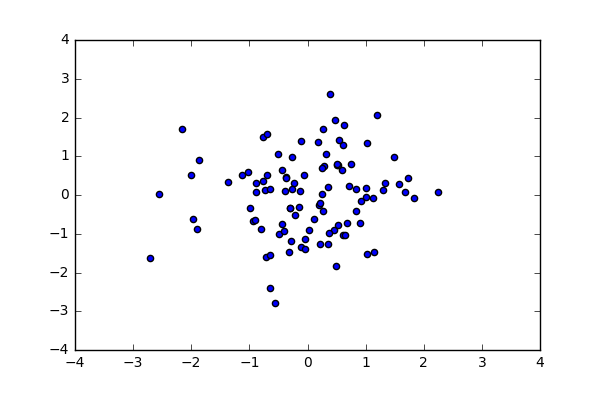
\includegraphics[width=0.4\textwidth]{hw1_8_1.png}
	       \captionsetup{labelformat=empty}
	       \caption{fig 8.1}
	       \label{fig:my_label}
	   \end{figure}
	\end{soln}
\item Make a scatter plot with a changed mean of $(1, -1)^T$.\\
	\begin{soln}
	   \begin{figure}[H]
	       \centering
	       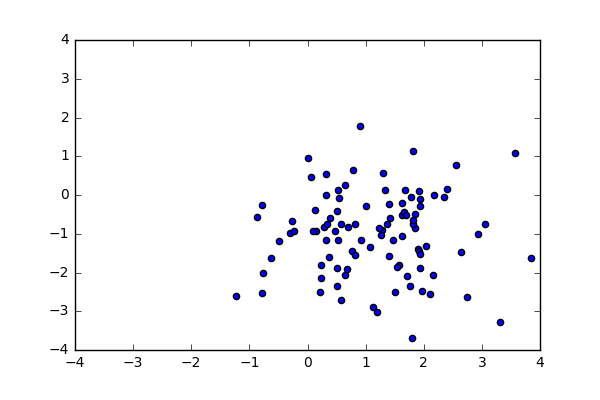
\includegraphics[width=0.4\textwidth]{hw1_8_2.png}
	       \captionsetup{labelformat=empty}
	       \caption{fig 8.2}
	       \label{fig:my_label}
	   \end{figure}
	\end{soln}
\item Make a scatter plot with a changed covariance matrix of $\begin{pmatrix}
    2 & 0 \\ 0 & 2\\
  \end{pmatrix}$.\\
  	\begin{soln}
	   \begin{figure}[H]
	       \centering
	       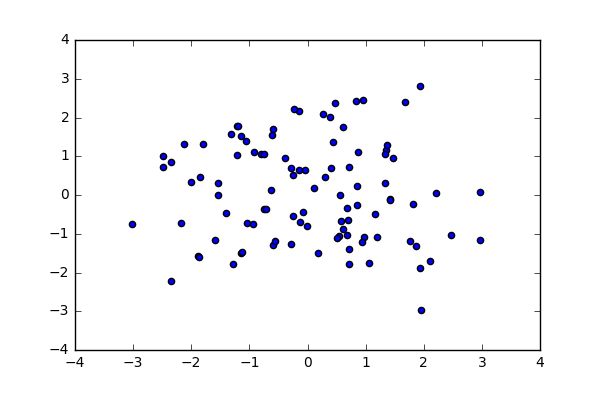
\includegraphics[width=0.4\textwidth]{hw1_8_3.png}
	       \captionsetup{labelformat=empty}
	       \caption{fig 8.3}
	       \label{fig:my_label}
	   \end{figure}
	\end{soln}
\item Make a scatter plot with a changed covariance matrix of $\begin{pmatrix}
    2 & 0.2 \\ 0.2 & 2\\
  \end{pmatrix}$.\\
  	\begin{soln}
	   \begin{figure}[H]
	       \centering
	       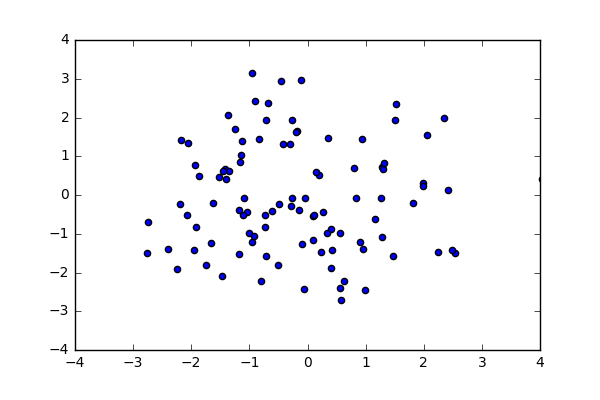
\includegraphics[width=0.4\textwidth]{hw1_8_4.png}
	       \captionsetup{labelformat=empty}
	       \caption{fig 8.4}
	       \label{fig:my_label}
	   \end{figure}
	\end{soln}
\item Make a scatter plot with a changed covariance matrix of $\begin{pmatrix}
    2 & -0.2 \\ -0.2 & 2\\
  \end{pmatrix}$.	\\
  	\begin{soln}
	   \begin{figure}[H]
	       \centering
	       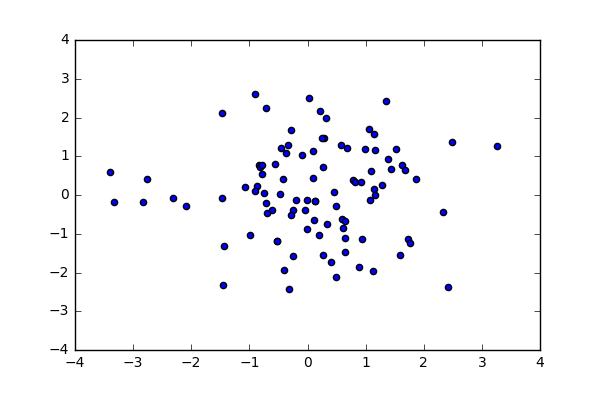
\includegraphics[width=0.4\textwidth]{hw1_8_5.png}
	       \captionsetup{labelformat=empty}
	       \caption{fig 8.5}
	       \label{fig:my_label}
	   \end{figure}
	\end{soln}
\end{enumerate}


\bibliographystyle{apalike}


%----------------------------------------------------------------------------------------


\end{document}
